%%%%%%%%%%%%%%%%%%%%%%%%%%%%%%%%%%%%%%%%%%%%%%%%%%%%%%%%%%%%%%%%%%
\begin{figure}[t!]
\centerline{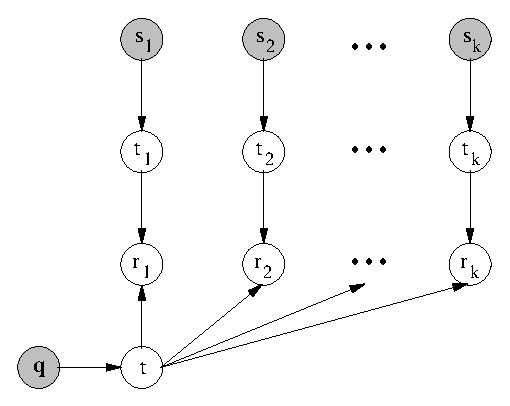
\includegraphics[scale = .8]{graphicalModel}}
\vspace{-2mm}
\caption{Latent subtopic binary relevance model.}
\vspace{-3mm}
\label{fig:gm}
\end{figure}
%%%%%%%%%%%%%%%%%%%%%%%%%%%%%%%%%%%%%%%%%%%%%%%%%%%%%%%%%%%%%%%%%%

In this article, we motivate diversity through the task of subtopic
retrieval~\cite{zhai03Beyond}.  Subtopics may differ according to a
variety of \emph{information needs}~\cite{diversity_types} such as
query facets (e.g., different political party views in a set of
blogs) or different ambiguous query interpretations (e.g.,
\emph{Java} the programming language vs. \emph{Java} the island).
%Subtopics may represent either
%\emph{intrinsic} information needs~\cite{diversity_types} such as
%query facets (e.g., the desire to see a variety of political positions
%in blog articles on a given topic) or \emph{extrinsic} information
%needs~\cite{diversity_types} such as ambiguous interpretations (e.g.,
%\emph{Java} the programming language vs. \emph{Java} the island).

We propose a directed graphical model (i.e., a Bayesian network) in
Figure~\ref{fig:gm} to formalize the independence assumptions in a
probabilistic subtopic model of binary relevance.  In
Figure~\ref{fig:gm}, shaded nodes represent observed variables,
whereas unshaded nodes are latent. The observed variables are the
query terms $\vec{q}$ and selected items $s_i$ (where for $1 \leq i
\leq k$, $s_i\in D$).  For the subtopic variables, let $T$ be a finite
and discrete subtopic set.  Then $t_i \in T$ represent subtopics for
respective $s_i$ and $t \in T$ represents a subtopic for query
$\vec{q}$.  The $r_i$ are binary variables that indicate if respective
selected items $s_i$ are relevant ($r_i=1$).

The conditional probability tables (CPTs) associated with each node in
Figure~\ref{fig:gm} are defined as follows: $P(t_i|s_i)$ and
$P(t|\vec{q})$ respectively represent the subtopic distribution for
item $s_i$ and query $\vec{q}$.  
%In this article, we are agnostic as
%to the source of this subtopic distribution for each document and
%query -- we need only assume they exist.  
The remaining CPTs are for
the relevance variables $r_i$; using $\I[\cdot]$ as a $\{0,1\}$
indicator function (1 if $\cdot$ is true), item $s_i$ is deemed
\emph{relevant} \emph{iff} \emph{its subtopic $t_i$ matches query
  subtopic $t$}:
\begin{align*}
P(r_{i}=1|t, t_{i}) & \; = \; \I[t_{i} = t]
\end{align*}
Here, $\I[\cdot]$ is $1$ when its argument is true and $0$ otherwise.

%The \emph{expected 1-call@$k$} objective is defined below: 
%\begin{align}
%\label{eq:setRelevance}
%    \ExpOneCall(S_k,\vec{q}) & = \mathbb{E} \left[\left. \bigvee_{i=1}^{k}r_i=1 \right| s_{1},\dots, s_{k},\vec{q} \right], 
%\end{align}

Given the specification of our latent subtopic binary relevance model,
we now formally define the expectation of $n$-call@$k$ w.r.t.\ this
model.  To facilitate this, we first define $R_k = \sum_{i=1}^k r_i$,
where $R_k$ is the number of relevant items from the first $k$
selections.  Interpreting $R_k \geq n$ as an indicator random variable
$\I[R_k \geq n]$, we can then express the \emph{expected $n$-call@$k$}
objective simply as
\begin{align}
\label{eq:setRelevance}
  \ExpNCall{n}(S_k,\vec{q})
  = \mathbb{E}[R_k\geq n|s_1,\dots,s_k,\vec{q}] .  
\end{align}
With our relevance model and objective now formally defined, 
we present our main theoretical results in the following section.
